\part{The algorithm}

%%%%%%%%%%%%%%%%%%%%%%%%%%%%%%%%%%%%%%%%%%%%%%%%%%%%%%%%%%%%%%%%%%%%%%%%%%%%%%%%%%%%%%%%%%%%%%%%%%%%%%%%%%%%%%%%%%%%%%%%%%%
%%%%%%%%%%%%%%%%%%%%%%%%%%%%%%%%%%%%%%%%%%%%%%%%%%%%%%%%%%%%%%%%%%%%%%%%%%%%%%%%%%%%%%%%%%%%%%%%%%%%%%%%%%%%%%%%%%%%%%%%%%%

\begin{frame}
	\partpage
	\centering
\end{frame}

%%%%%%%%%%%%%%%%%%%%%%%%%%%%%%%%%%%%%%%%%%%%%%%%%%%%%%%%%%%%%%%%%%%%%%%%%%%%%%%%%%%%%%%%%%%%%%%%%%%%%%%%%%%%%%%%%%%%%%%%%%%
%%%%%%%%%%%%%%%%%%%%%%%%%%%%%%%%%%%%%%%%%%%%%%%%%%%%%%%%%%%%%%%%%%%%%%%%%%%%%%%%%%%%%%%%%%%%%%%%%%%%%%%%%%%%%%%%%%%%%%%%%%%

\begin{frame}
	\frametitle{Naive algorithm}
	\centering
	
	\begin{itemize}
	  \item Store all $(k+1)$-mers in a hash table
	  \item For each $k$-mers query the possible edge
	  \item If only 1 in and 1 out edge, unmark as a junction
	\end{itemize}
	   
	\medskip
	
   \scalebox{.55}{                        
   \begin{algorithm}[H]
      \small
       \DontPrintSemicolon
       \SetKwInOut{Input}{Input}
       \SetKwInOut{Output}{Output}
       \Input{strings $S = \{s_{1}, ..., s_{m}\}$ genoma sequences\\integer $k$, size of $k$-mers\\ Candidate set of junctions $C_{in}$ (\textbf{for now all positions are marked})}
       \Output{A reduce candidate set of junctions $C$}
       
       \BlankLine
       \ForEach{$s \in S$}{
        \For{$1 \leq i < |s| - k $}{
          \If{$C[s,i] = marked$}{ 
            $E \gets E \cup  s[i..i+k] \cup  s[i-1..i+k-1]$ \Comment*[r]{Store all $(k+1)$-mers}
          }
        }
       }
       \BlankLine
       \ForEach{$s \in S$}{
        \For{$1 \leq i < |s| - k $}{
          \If{$C[s,i] = marked$}{
          
            $(in, out) \gets (0, 0)$ \Comment*[r]{Count in/out edges}
            
            \ForEach{$c \in \{A, C, G, T\}$}{
              \If{$v \cdot c \in E$}{
                $in \gets in + 1$\;
              }
              \If{$c \cdot v \in E$}{
                $out \gets out + 1$\;
              }
            }
            
            \If{$(in, out) = (1,1)$}{
              $C[s,i] = unmarked$ \Comment*[r]{surely not a junction}
            }
          }
        }
       }
              
       \Return{$C$}
       \caption{\textsc{Filter-Junctions}}
   \end{algorithm}
   }
   
\end{frame}

%%%%%%%%%%%%%%%%%%%%%%%%%%%%%%%%%%%%%%%%%%%%%%%%%%%%%%%%%%%%%%%%%%%%%%%%%%%%%%%%%%%%%%%%%%%%%%%%%%%%%%%%%%%%%%%%%%%%%%%%%%%
%%%%%%%%%%%%%%%%%%%%%%%%%%%%%%%%%%%%%%%%%%%%%%%%%%%%%%%%%%%%%%%%%%%%%%%%%%%%%%%%%%%%%%%%%%%%%%%%%%%%%%%%%%%%%%%%%%%%%%%%%%%

\begin{frame}
	\frametitle{The memory issue}
	
	  First part of the naive algorithm:
	  
	  \bigskip
	  
	  \ForEach{$s \in S$}{
      \For{$1 \leq i < |s| - k $}{
          \If{$C[s,i] = marked$}{
            $E \gets E \cup  s[i..i+k] \cup  s[i-1..i+k-1]$\;
        }
      }
    }
     
	 \centering

    \bigskip

    We don't really need and, in almost all pratical cases, \\ we can't store all the possible $(k+1)$-mers.
    
    \bigskip
    
    Mainly because \textbf{only a little percentual} of them are \\ junction in the de Bruijn graph.
      
\end{frame}

%%%%%%%%%%%%%%%%%%%%%%%%%%%%%%%%%%%%%%%%%%%%%%%%%%%%%%%%%%%%%%%%%%%%%%%%%%%%%%%%%%%%%%%%%%%%%%%%%%%%%%%%%%%%%%%%%%%%%%%%%%%
%%%%%%%%%%%%%%%%%%%%%%%%%%%%%%%%%%%%%%%%%%%%%%%%%%%%%%%%%%%%%%%%%%%%%%%%%%%%%%%%%%%%%%%%%%%%%%%%%%%%%%%%%%%%%%%%%%%%%%%%%%%

\begin{frame}
	\frametitle{Bloom filter}
	
	\centering

	A space-efficient probabilistic hash table
	
	\medskip
	
	Bitmap $V$ of size $b$, $h$ hash functions $f_{0}, f_{1}, ..., f_{h-1} : U \rightarrow [0, b-1]$ \\
		
	\medskip
	
	insertion($x$) $\rightarrow V[f_{i}(x)] = 1$, $\forall$ $0 \leq i < h$ 
	
	\medskip
	
	contains($x$) $\rightarrow$ \textbf{probabily yes} if $V[f_{i}(x)] == 1$, $\forall$ $0 \leq i < h$
  \medskip
  
  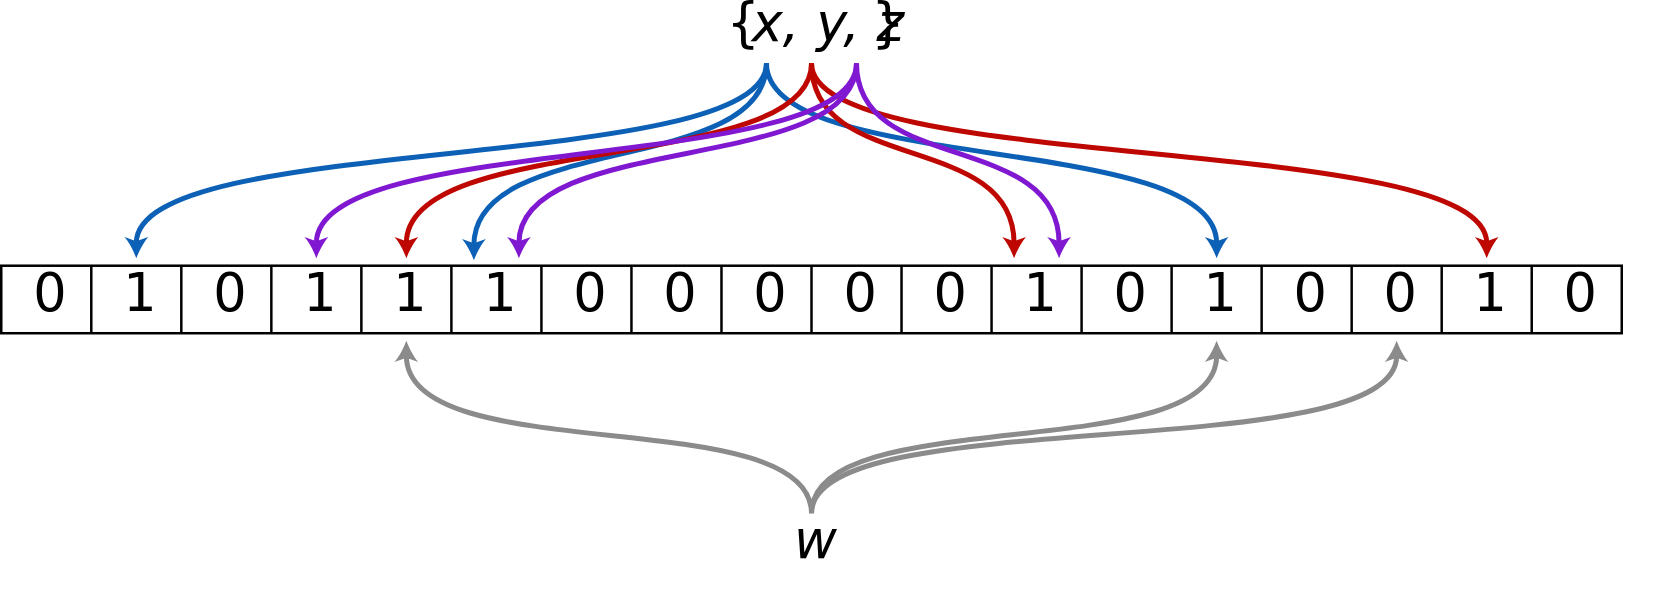
\includegraphics[height=3cm]{images/bloom_filter}
  
  \medskip
	Probability of false positive, after $n$ insertion: $p_{FP} \simeq (1 - e^{-hn/m})^{h}$
	
	
\end{frame}

%%%%%%%%%%%%%%%%%%%%%%%%%%%%%%%%%%%%%%%%%%%%%%%%%%%%%%%%%%%%%%%%%%%%%%%%%%%%%%%%%%%%%%%%%%%%%%%%%%%%%%%%%%%%%%%%%%%%%%%%%%%
%%%%%%%%%%%%%%%%%%%%%%%%%%%%%%%%%%%%%%%%%%%%%%%%%%%%%%%%%%%%%%%%%%%%%%%%%%%%%%%%%%%%%%%%%%%%%%%%%%%%%%%%%%%%%%%%%%%%%%%%%%%

\begin{frame}
	\frametitle{Two Pass version}
	\centering
	
	\begin{itemize}
	  \item First pass: Select a set of junction candidates by insert all the $(k+1)$-mers in a bloom filter of choosing size
	  \item Second pass: Filter out the false positive by storing the reduce sets of $(k+1)$-mers in an hash table
	\end{itemize}

   \scalebox{.8}{                        
   \begin{algorithm}[H]
      \small
       \DontPrintSemicolon
       \SetKwInOut{Input}{Input}
       \SetKwInOut{Output}{Output}
       \Input{strings $S = \{s_{1}, ..., s_{m}\}$ genoma sequences\\integer $k$, size of $k$-mers\\integer $b$, size of bloom filter\\ Candidate set of junctions $C_{in}$}
       \Output{A reduce candidate set of junctions $C_{out}$}
       
       \BlankLine
       
       $F \gets$ empty bloom filter of size $b$ \Comment*[r]{First pass}
       $C_{temp} \gets \textsc{Filter-Junctions}(S, k, F, C_{in})$  \;

       \BlankLine

       $H \gets$ empty hash table \Comment*[r]{Second pass}
       $C_{out} \gets \textsc{Filter-Junctions}(S, k, H, C_{in})$ \;

       \BlankLine
              
       \Return{$C_{out}$}
       \caption{\textsc{Filter-Junctions-Two-Pass}}
   \end{algorithm}
   }
   

\end{frame}

%%%%%%%%%%%%%%%%%%%%%%%%%%%%%%%%%%%%%%%%%%%%%%%%%%%%%%%%%%%%%%%%%%%%%%%%%%%%%%%%%%%%%%%%%%%%%%%%%%%%%%%%%%%%%%%%%%%%%%%%%%%
%%%%%%%%%%%%%%%%%%%%%%%%%%%%%%%%%%%%%%%%%%%%%%%%%%%%%%%%%%%%%%%%%%%%%%%%%%%%%%%%%%%%%%%%%%%%%%%%%%%%%%%%%%%%%%%%%%%%%%%%%%%

\begin{frame}
	\frametitle{The memory issue$^{2}$}
	\centering
\end{frame}

%%%%%%%%%%%%%%%%%%%%%%%%%%%%%%%%%%%%%%%%%%%%%%%%%%%%%%%%%%%%%%%%%%%%%%%%%%%%%%%%%%%%%%%%%%%%%%%%%%%%%%%%%%%%%%%%%%%%%%%%%%%
%%%%%%%%%%%%%%%%%%%%%%%%%%%%%%%%%%%%%%%%%%%%%%%%%%%%%%%%%%%%%%%%%%%%%%%%%%%%%%%%%%%%%%%%%%%%%%%%%%%%%%%%%%%%%%%%%%%%%%%%%%%

\begin{frame}

	\frametitle{Multiple rounds: dealing with memory restrictions}
	\centering
	
	\begin{itemize}
	  \item Partitionate input $k$-mers in 
	  \item 
	\end{itemize}

\end{frame}

%%%%%%%%%%%%%%%%%%%%%%%%%%%%%%%%%%%%%%%%%%%%%%%%%%%%%%%%%%%%%%%%%%%%%%%%%%%%%%%%%%%%%%%%%%%%%%%%%%%%%%%%%%%%%%%%%%%%%%%%%%%
%%%%%%%%%%%%%%%%%%%%%%%%%%%%%%%%%%%%%%%%%%%%%%%%%%%%%%%%%%%%%%%%%%%%%%%%%%%%%%%%%%%%%%%%%%%%%%%%%%%%%%%%%%%%%%%%%%%%%%%%%%%

\begin{frame}
	\frametitle{Parallelization scheme}
	\centering
\end{frame}
